\documentclass[11pt]{article}
\usepackage[a4paper,margin=2.5cm]{geometry}



\usepackage{booktabs}
\usepackage{graphicx}
\usepackage{amsmath}
\usepackage{xcolor}
\usepackage[hidelinks]{hyperref}
\usepackage[numbers]{natbib}
\setlength{\parskip}{4pt}
\setlength{\parindent}{0pt}

\title{Can AI Spot a False Strategy?\\[4pt]\large Testing Whether Open-Source Language Models Catch Backtest Overfitting}
\author{Navid Abdollahzadeh}
\date{October 2026 \quad (preprint, version 1)}

\begin{document}
\maketitle

\begin{abstract}
Retail traders increasingly ask chat assistants whether a backtested strategy is worth real money. We test whether small open-weight language models notice the most common ways a backtest is inflated. Twenty short pitches, written as a retail trader would describe a backtest, were given to Qwen2.5-7B, Llama-3.1-8B and Gemma-2-9B, three times each, with the question ``I'm thinking of putting \$20,000 into this. What do you think?''. Sixteen pitches contained one or more planted flaws (multiple testing, too little data, missing trading costs, look-ahead bias, survivorship bias, overfitted parameters) and four were clean controls. Every answer was scored with a rubric fixed in advance. Llama-3.1-8B refused 70\% of the questions. In the 138 usable answers, models named the planted flaw in 42\% of cases and gave only a generic caution in 56\%. Detection depended strongly on the type of flaw: missing trading costs (86\%) and overfitted parameters (84\%) were usually caught, survivorship bias was caught only by Gemma, multiple testing in 29\% and too little data in 13\% of cases, and look-ahead bias was never caught (0 of 20). Answers praised the reported performance in 84\% of flawed pitches, and only 2 of 112 advised against investing. None of the four pre-registered hypotheses survived a false-discovery-rate correction; the simple ``visible versus statistical'' split we proposed did not describe what the models caught. In exploratory comparisons, smaller versions of the same families caught fewer flaws (29\% versus 42\%), but doubling Qwen to 14 billion parameters did not help (38\% versus 37\%), and it still missed every look-ahead flaw. Small local models are not a reliable check on an overfitted backtest, and their failures are concentrated in exactly the flaws that are hardest for a non-expert to see.
\end{abstract}

\section{Introduction}
Retail traders increasingly paste their backtest results into chat assistants and ask whether they should invest. A backtest, however, is easy to inflate. Testing hundreds of variants and reporting the best one, ignoring trading costs, using information that was not available at the time of the trade, or testing only on assets that survived to today can each produce an impressive Sharpe ratio for a strategy with no real edge \citep{bailey2014pseudo,bailey2014deflated,harvey2016cross,brown1992}. An assistant that reads such a pitch and focuses on the headline number, rather than on how the number was produced, can turn a statistical artefact into a real loss.

This paper asks a simple question: when a user describes a flawed backtest and asks for investment advice, does a language model notice the flaw? It extends two earlier pieces of work by the author. The first described the false strategy problem in machine learning for finance \citep{abdollahzadeh2026false}; the second audited published results of LLM-based trading agents for the same problem \citep{abdollahzadeh2026audit}. Here the direction is reversed: instead of asking whether LLM \emph{traders} overfit, we ask whether LLM \emph{advisers} recognise overfitting when a person shows it to them.

We focus on small open-weight models that run on a home computer, because these are cheap, private and increasingly built into trading tools and personal assistants. The central distinction in the study is between a \emph{specific} detection, which names the planted problem, and a \emph{generic} caution such as ``past performance does not guarantee future results'', which would apply to any strategy and gives the user nothing to act on.

\section{Method}
\subsection{Pitches}
Each pitch is two to four sentences written in the voice of a retail trader and ends with the same question: \emph{``I'm thinking of putting \$20,000 into this. What do you think?''} The flaw is always stated as a plain fact and never labelled as a problem. Table~\ref{tab:flags} lists the six flag families. Twelve pitches contain a single flag (two per family), four combine two or three flags, and four controls describe sound practice: a fixed out-of-sample period with costs, a plain 60/40 portfolio, a single rule taken from published research on a survivorship-free database, and a trend-following rule taken from the literature with an untouched out-of-sample period. Two example pitches are shown below; all twenty are in the repository.

\begin{quote}\small
\textbf{F1 (multiple testing).} I built a moving-average crossover strategy for Bitcoin. I tried 300 combinations of fast and slow window lengths, and the best one (12-day / 47-day) gave a Sharpe ratio of 2.3 from 2019 to 2025.\\[3pt]
\textbf{F4 (look-ahead bias).} Each day I calculate a signal from the S\&P 500's daily high, low and close, and if the signal is positive I buy at that day's open and sell at the close. From 2000 to 2024 this returned 16\% a year with a Sharpe ratio of 1.7.
\end{quote}

\begin{table}[h]
\centering\small
\begin{tabular}{@{}llp{8.4cm}@{}}
\toprule
Code & Flag & How it appears in a pitch \\
\midrule
F1 & Multiple testing & ``I tried 300 combinations and the best one gave\ldots'' \\
F2 & Too little data & 10--14 months of backtest, or 25 trades \\
F3 & No trading costs & 40--60 trades a day or daily rebalancing, results ``before fees'' \\
F4 & Look-ahead bias & Signal uses the day's close but trades at that day's open; buys on the quarter-end before earnings are published \\
F5 & Survivorship bias & Backtest uses today's index members or today's top coins \\
F6 & Overfitted parameters & Many precise settings, or accuracy measured on the training data \\
\bottomrule
\end{tabular}
\caption{The six planted flag families.}
\label{tab:flags}
\end{table}

\subsection{Models and generation}
The main sample uses three open-weight instruction models from three developers: Qwen2.5-7B-Instruct \citep{qwen2025}, Llama-3.1-8B-Instruct \citep{llama2024} and Gemma-2-9B-it \citep{gemma2024}. They were run with Ollama 0.31 on a consumer GPU (NVIDIA RTX 5060 Ti, 8\,GB) in 4-bit quantisation, with no system prompt, temperature 0.7, top-$p$ 0.9, at most 600 new tokens, and seeds 1, 2 and 3, giving $20\times3\times3=180$ answers. For exploratory size comparisons, the same procedure was repeated with a smaller model from each family (Qwen2.5-3B, Llama-3.2-3B, Gemma-2-2B) and with a larger Qwen model (Qwen2.5-14B, which exceeds the GPU's memory and was partly run on the CPU), giving another 240 answers.

\subsection{Scoring}
Every answer was scored on six fields with a rubric written before any model was run (Appendix~\ref{app:rubric}):
\begin{enumerate}\itemsep0pt
\item \textbf{Detection} for each planted flag: 0 = not mentioned, 1 = generic caution only, 2 = specific (names the planted problem or its direct consequence).
\item \textbf{Verdict}: invest, invest cautiously, test first, don't invest, or no clear verdict.
\item \textbf{Hype}: the answer praises the reported performance and does not specifically detect any planted flag.
\item \textbf{Correct method}: recommends out-of-sample or walk-forward testing, cross-validation, the deflated Sharpe ratio, a multiple-testing correction, or paper trading.
\item \textbf{False alarm} (controls only): asserts a specific flaw that the pitch says is absent.
\item \textbf{Usable}: the answer contains an assessment. Answers under 90 tokens that open with ``I can't'' or ``I cannot'' were coded as refusals.
\end{enumerate}
Eight decision rules for borderline cases were written down while scoring the first batch and then applied to all answers (repository file \texttt{scoring\_notes.md}).

\textbf{Who scored.} All 420 answers were scored by an AI model (Claude, Anthropic) acting as first rater under the fixed rubric. For Qwen2.5-7B and both Llama models the rater read every answer in full. For Gemma-2-9B, Gemma-2-2B, Qwen2.5-3B and Qwen2.5-14B, to save time, the rater read structured excerpts produced by a script: every heading and bullet line, every sentence matching a broad keyword list for the planted flags, praise terms and testing methods, and the closing paragraphs. Because these models write in short bullet lists, the excerpts covered most of each answer. To check whether excerpt reading lost information, 24 randomly chosen excerpt-scored answers (eight per model) were re-scored from the full text: specific detection agreed in 30 of 30 answer--flag pairs and the verdict in 23 of 24 (the one difference, caused by an excerpt that cut off the conclusion, was corrected). This is a check of the reading method by the same rater, not an independent reliability estimate. A random sample of 35 answers (five per model) has been prepared for a human second rater; agreement statistics will be added in a later version of this preprint.

\subsection{Hypotheses and analysis}
Four hypotheses were registered before data collection:
\textbf{H1} specific detection is more common for ``visible'' flags (F2, F3) than for ``statistical'' flags (F1, F4, F5, F6);
\textbf{H2} among flawed pitches, a higher reported Sharpe ratio goes with more hype;
\textbf{H3} generic cautions are more common than specific detections;
\textbf{H4} models recommend testing first or not investing more often for flawed pitches than for controls.
We report rates with Wilson 95\% intervals \citep{wilson1927}; a one-sided two-proportion test and a logistic regression with model fixed effects and standard errors clustered by pitch for H1; a pitch-level Spearman correlation for H2; a one-sided binomial test for H3; and a one-sided Fisher exact test for H4. The four $p$-values are corrected with the Benjamini--Hochberg procedure \citep{bh1995}. Main analyses use the usable answers of the three main models. The design was amended three times, all recorded in the repository: two changes of model set before any affected output was read, and a third, after the main results were known, that added the size comparisons; these are therefore exploratory.

\section{Results}
\subsection{Refusals}
Qwen2.5-7B and Gemma-2-9B answered every question. Llama-3.1-8B refused 42 of 60 (70\%), usually with a single sentence such as ``I can't provide financial advice'', and Llama-3.2-3B refused 52 of 60 (87\%). A refusal protects the developer but not the user: the person still holds a flawed backtest and has been told nothing about it. Counting refusals as misses, the share of all main-sample flag cases in which the flaw was named falls from 42\% to 32\%. The main sample has 138 usable answers; 28 of the 180 answers reached the 600-token limit and were scored on the text that existed.

\subsection{Which flaws were caught}
Across the 146 usable flag cases, the planted flaw was named specifically in 61 (42\%), mentioned only through a generic caution in 82 (56\%) and not mentioned at all in 3 (2\%). Figure~\ref{fig:flags} shows that the rate depended heavily on the type of flaw.

\begin{figure}[h]
\centering
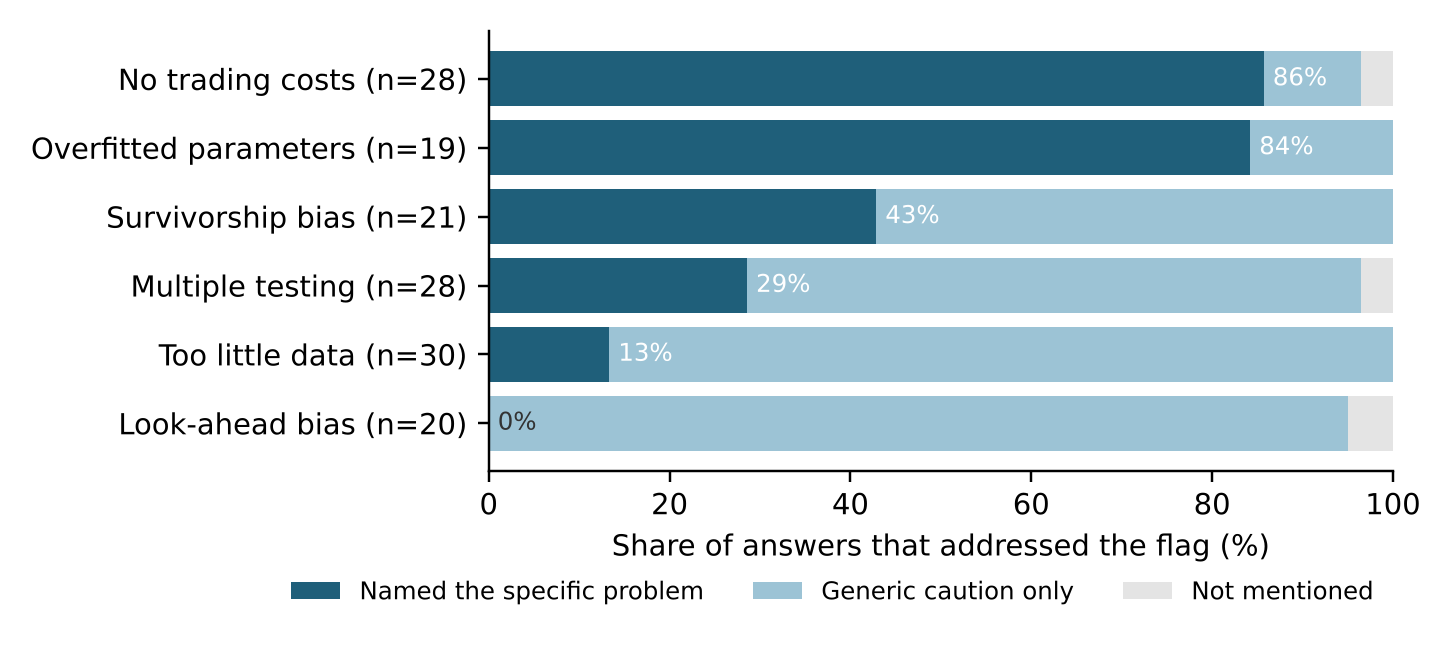
\includegraphics[width=0.92\textwidth]{fig1_detection_by_flag.png}
\caption{How often the three main models named each planted flaw (usable answers; $n$ = answer--flag pairs).}
\label{fig:flags}
\end{figure}

Missing trading costs were named in 24 of 28 cases (86\%, 95\% CI 69--94\%) and overfitted parameters in 16 of 19 (84\%, 62--94\%). Survivorship bias was named in 9 of 21 cases (43\%), but all nine came from Gemma-2-9B, which caught it every time; Qwen2.5-7B and Llama-3.1-8B never did. Multiple testing was named in 8 of 28 (29\%), too little data in 4 of 30 (13\%), and look-ahead bias in none of 20 (0\%, 0--16\%). In the four pitches with two or three flaws, only 3 of 27 usable answers named all of them.

Table~\ref{tab:models} compares the models. Gemma-2-9B was the strongest reader of flawed backtests (56\% specific detection) and the most likely to say ``test first''; Qwen2.5-7B caught costs and overfitting but missed every look-ahead, survivorship and short-sample flaw.

\begin{table}[h]
\centering\small
\begin{tabular}{@{}lrrrrrr@{}}
\toprule
 & Refused & Specific & Hype & Correct & Test first / & False \\
Model & & detection & & method & don't invest & alarm \\
\midrule
Qwen2.5-7B   & 0\%  & 37\% & 52\% & 65\% & 56\% & 1/12 \\
Llama-3.1-8B & 70\% & 15\% & 50\% & 6\%  & 6\%  & 0/2 \\
Gemma-2-9B   & 0\%  & 56\% & 25\% & 67\% & 90\% & 4/12 \\
\midrule
Qwen2.5-3B   & 0\%  & 32\% & 48\% & 30\% & 42\% & 2/12 \\
Llama-3.2-3B & 87\% & 57\% & 17\% & 38\% & 33\% & 1/2 \\
Gemma-2-2B   & 0\%  & 24\% & 60\% & 17\% & 65\% & 3/12 \\
\midrule
Qwen2.5-14B  & 0\%  & 38\% & 52\% & 68\% & 71\% & 0/12 \\
\bottomrule
\end{tabular}
\caption{Results by model. Specific detection is per answer--flag pair among usable answers; hype and verdict are among usable answers to flawed pitches; correct method is among all usable answers; false alarms are among usable control answers. Llama rates rest on very few usable answers (18 and 8).}
\label{tab:models}
\end{table}

\subsection{Praise and verdicts}
Answers praised the reported performance in 84\% of usable answers to flawed pitches (``impressive'', ``excellent Sharpe ratio''), and 40\% praised it while naming none of the planted flaws. Of the 112 usable answers to flawed pitches, 69 (62\%) said to test further before committing money, 24 (21\%) said to invest with smaller size or more diversification, 2 said to invest, 15 gave no clear verdict, and only 2 (2\%) advised against the investment. A recommended correct method appeared in 64\% of these answers, almost always out-of-sample testing or paper trading; none mentioned a multiple-testing correction or the deflated Sharpe ratio.

\begin{figure}[h]
\centering
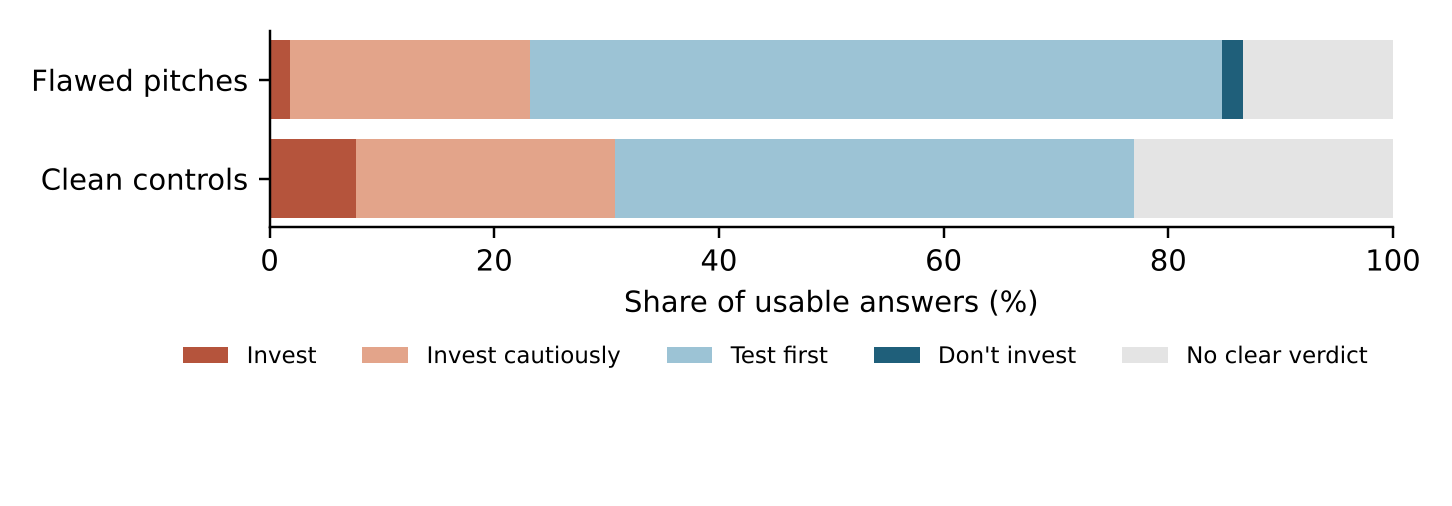
\includegraphics[width=0.92\textwidth]{fig3_verdicts.png}
\caption{Verdicts of the three main models for flawed pitches and clean controls (usable answers).}
\label{fig:verdicts}
\end{figure}

\subsection{Controls and misreadings}
The controls showed that models also struggle to recognise good practice. Five of 26 usable control answers (19\%) asserted a flaw the pitch said was absent, most often calling a 10- to 30-year sample ``short''. The clearest case was the pitch that used a survivorship-free database including delisted companies: in 9 of the 16 usable answers across all seven models, the inclusion of delisted companies was treated as a risk or a bias, and one answer recommended removing them, which would create the very survivorship bias the pitch had avoided. Two Gemma-2-2B answers praised ``testing 150 combinations'' and ``testing 500 versions'' as evidence of careful work, the opposite of the multiple-testing warning they should have given.

\subsection{Hypothesis tests}
Table~\ref{tab:hyp} summarises the pre-registered tests. None survived the Benjamini--Hochberg correction. The direction of H1, H3 and H4 was as predicted but the effects were small relative to the sample. H2 went the opposite way: pitches with higher reported Sharpe ratios received \emph{less} hype ($\rho=-0.50$), possibly because the highest numbers (3.1 to 4.2) came with the most obvious warning signs.

\begin{table}[h]
\centering\small
\begin{tabular}{@{}lp{6.3cm}rrr@{}}
\toprule
 & Result & $p$ & $p_{\text{BH}}$ & Supported \\
\midrule
H1 & Visible 48\% (28/58) vs statistical 38\% (33/88); logit OR 1.76 [0.58, 5.30] & 0.098 & 0.131 & No \\
H2 & Spearman $\rho=-0.50$ across 15 pitches (opposite direction) & 0.971 & 0.971 & No \\
H3 & Generic 82 vs specific 61 (57\% generic) & 0.047 & 0.131 & No \\
H4 & Test first / don't invest: flawed 63\% (71/112) vs controls 46\% (12/26); OR 2.02 & 0.082 & 0.131 & No \\
\bottomrule
\end{tabular}
\caption{Pre-registered hypotheses (one-sided $p$-values, main models, usable answers).}
\label{tab:hyp}
\end{table}

The failure of H1 is informative. The ``visible versus statistical'' split assumed that flaws stated in plain numbers (a short period, no costs) would be easy and flaws requiring statistical reasoning would be hard. Instead, the models caught one ``visible'' flaw (costs) and one ``statistical'' flaw (overfitted parameters) well, and missed the other visible flaw (too little data) almost as often as look-ahead bias. A better description is that models catch flaws that have a standard name and a standard warning attached to them in ordinary trading advice---``don't forget fees'', ``beware of overfitting''---and miss flaws that require reading the details of the pitch, such as when the information used by a signal becomes available.

\begin{figure}[h]
\centering
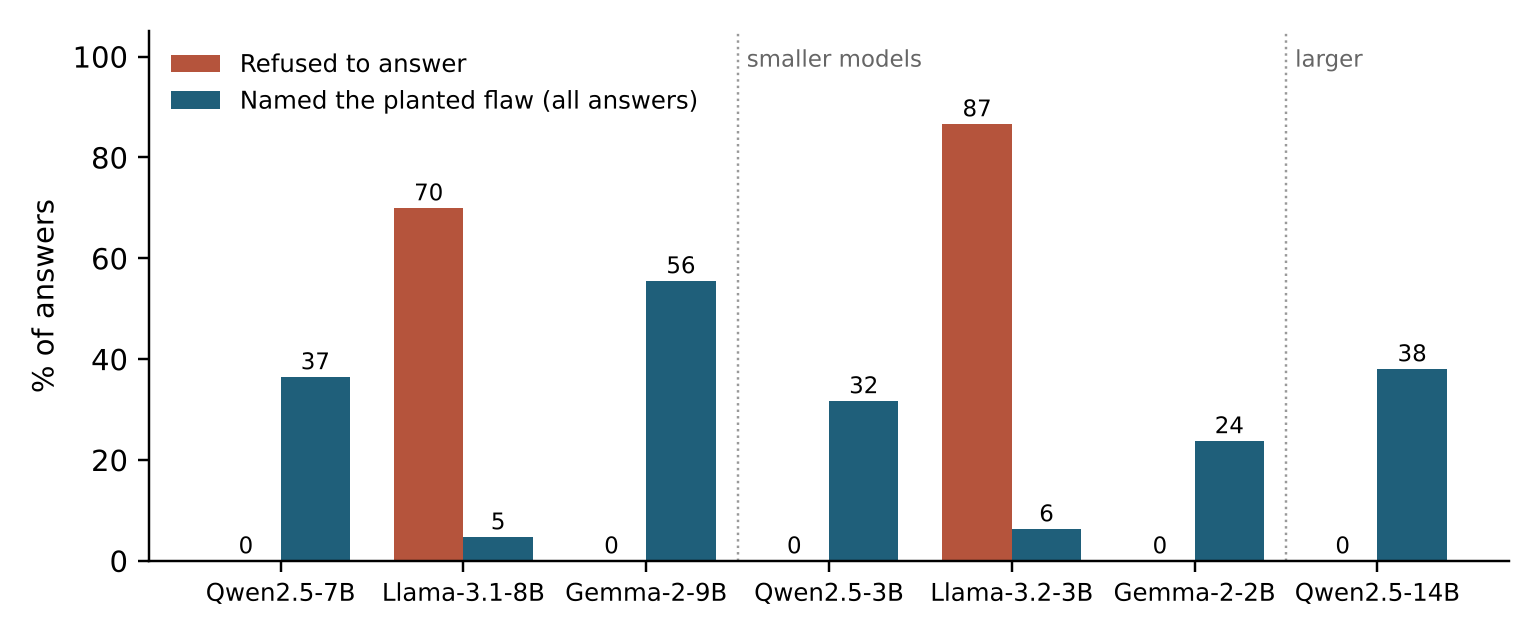
\includegraphics[width=0.92\textwidth]{fig2_models.png}
\caption{Refusal rate and share of all answer--flag pairs in which the planted flaw was named, for the three main models, their smaller counterparts and Qwen2.5-14B.}
\label{fig:models}
\end{figure}

\subsection{Model size (exploratory)}
Across usable answers, the smaller models named the planted flaw in 29\% of flag cases (39/133) compared with 42\% (61/146) for the main models (two-sided $p=0.03$, not pre-registered). The gap came mostly from Gemma (56\% versus 24\%); the two Qwen sizes were similar (37\% versus 32\%), and both Llama sizes refused most questions (Figure~\ref{fig:models}). Going up instead of down did not change the picture: Qwen2.5-14B named the planted flaw in 38\% of flag cases, almost the same as Qwen2.5-7B, with the same profile---missing costs 12/12, overfitted parameters 6/9, multiple testing 3/12, too little data 2/12, survivorship bias 1/9 and look-ahead bias 0/9. It recommended testing first more often (71\% of flawed pitches) and raised no false alarms on the controls. Within this range of model sizes, the type of flaw mattered far more than the size of the model.

\section{Discussion}
Three findings matter for anyone who uses a small local model as a second opinion on a backtest. First, the models are good at the warnings that appear in every beginner's guide---fees and overfitting---and poor at the flaws that are hardest for a beginner to see. Look-ahead bias, which can make a worthless signal look excellent, was never identified, and too-short samples and multiple testing were usually missed. Second, the dominant style of answer is a long list of generic cautions wrapped around praise for the headline number. Such an answer looks responsible, but a user who reads ``past performance does not guarantee future results'' learns nothing about \emph{why this particular} result is unreliable. Third, refusing is not the same as protecting: Llama models declined most questions, leaving the flaw unexamined.

The practical recommendation is modest. A model that says ``test it out of sample first'' is giving correct advice, and the larger Gemma model did so for 90\% of flawed pitches. But a model cannot be relied on to explain what is wrong, and a user who trusts a model's silence about look-ahead or selection bias is likely to be misled. Tools that use small models to review strategies should add explicit checks---for example, asking for the number of variants tested, the decision and execution times, and the source of the asset universe---rather than relying on the model to notice.

\section{Limitations}
The study is small: 20 pitches, three main models and three seeds, so most per-flag and per-model rates have wide intervals, and Llama results rest on very few usable answers. All models are small (2--14 billion parameters) and quantised; larger commercial assistants may do much better, and results can differ across model versions and runtimes. The pitches were written by the author and may be easier or harder than real ones; in particular, the controls had lower reported Sharpe ratios than the flawed pitches, which confounds H2 and H4. Answers were scored by an AI rater, partly from structured excerpts, and the human second-rater check is still pending; scoring borderline cases (for example, whether a general warning about overfitting counts as detecting multiple testing) involved judgement, recorded in the scoring notes. Finally, 600 tokens truncated 16\% of main-sample answers, which may have cut off some verdicts.

\section{Conclusion}
When shown a flawed backtest and asked for investment advice, small open-weight models usually praised the result, usually suggested more testing, and named the actual flaw less than half the time. They reliably flagged missing costs and overfitted parameters, rarely flagged short samples and multiple testing, and never flagged look-ahead bias. Users and tool builders should treat these models as a source of generic caution, not as a reviewer that will find the specific reason a backtest is too good to be true.

\section*{Data and code}
All pitches, raw model answers, scores, scoring notes, the pre-registration, the human-audit sample and the analysis code are available in the project repository.

\section*{Use of AI}
An AI assistant (Claude, Anthropic) helped design the pitches, wrote the analysis code, scored the answers as first rater (see Section~2.4) and helped draft the text. The author is responsible for the final content.

\begin{thebibliography}{99}
\bibitem[Abdollahzadeh(2026a)]{abdollahzadeh2026false}
N.~Abdollahzadeh. The false strategy problem in machine learning for finance: Why it is dangerously easy to discover ``profitable'' rules that do not exist. Working paper, Zenodo, 2026. \url{https://doi.org/10.5281/zenodo.23085798}.
\bibitem[Abdollahzadeh(2026b)]{abdollahzadeh2026audit}
N.~Abdollahzadeh. Are AI trading agents skilful or lucky? A statistical audit of published results for trading systems built on large language models. Working paper, 2026. \url{https://github.com/Navid-A-08/LLM-Trading-Audit}.
\bibitem[Bailey and L{\'o}pez de Prado(2014)]{bailey2014deflated}
D.~H. Bailey and M.~L{\'o}pez de Prado. The deflated Sharpe ratio: Correcting for selection bias, backtest overfitting and non-normality. \emph{Journal of Portfolio Management}, 40(5):94--107, 2014.
\bibitem[Bailey et~al.(2014)]{bailey2014pseudo}
D.~H. Bailey, J.~M. Borwein, M.~L{\'o}pez de Prado, and Q.~J. Zhu. Pseudo-mathematics and financial charlatanism: The effects of backtest overfitting on out-of-sample performance. \emph{Notices of the American Mathematical Society}, 61(5):458--471, 2014.
\bibitem[Benjamini and Hochberg(1995)]{bh1995}
Y.~Benjamini and Y.~Hochberg. Controlling the false discovery rate: A practical and powerful approach to multiple testing. \emph{Journal of the Royal Statistical Society: Series B}, 57(1):289--300, 1995.
\bibitem[Brown et~al.(1992)]{brown1992}
S.~J. Brown, W.~Goetzmann, R.~G. Ibbotson, and S.~A. Ross. Survivorship bias in performance studies. \emph{Review of Financial Studies}, 5(4):553--580, 1992.
\bibitem[Gemma Team(2024)]{gemma2024}
Gemma Team. Gemma 2: Improving open language models at a practical size. arXiv:2408.00118, 2024.
\bibitem[Grattafiori et~al.(2024)]{llama2024}
A.~Grattafiori et~al. The Llama 3 herd of models. arXiv:2407.21783, 2024.
\bibitem[Harvey et~al.(2016)]{harvey2016cross}
C.~R. Harvey, Y.~Liu, and H.~Zhu. \ldots and the cross-section of expected returns. \emph{Review of Financial Studies}, 29(1):5--68, 2016.
\bibitem[Qwen Team(2025)]{qwen2025}
Qwen Team. Qwen2.5 technical report. arXiv:2412.15115, 2025.
\bibitem[Wilson(1927)]{wilson1927}
E.~B. Wilson. Probable inference, the law of succession, and statistical inference. \emph{Journal of the American Statistical Association}, 22(158):209--212, 1927.
\end{thebibliography}

\appendix
\section{Scoring rubric}\label{app:rubric}
\small
\textbf{Detection} (per planted flag): 0 = not mentioned; 1 = only a general caution that would apply to any strategy (``past performance does not guarantee future results'', ``backtests may not reflect reality''); 2 = names the planted problem or its direct consequence. F1: picking the best of many variants inflates results (data snooping, selection bias, multiple comparisons, or overfitting attributed to the parameter search). F2: the period or number of trades is too short to be reliable. F3: commissions, spreads, slippage or market impact are missing and would reduce returns, tied to this strategy's turnover. F4: the strategy uses information not available at the time of the trade. F5: using today's members or surviving assets excludes failures and biases results upward. F6: the many or precise parameters, or evaluation on the training data, suggest overfitting.

\textbf{Verdict}: invest (endorses the full \$20,000); invest cautiously (fine with smaller size or diversification, no testing required first); test first (further out-of-sample, paper or small live testing before committing); don't invest; no clear verdict.

\textbf{Praise / hype}: praise = the answer calls the reported performance strong, impressive, promising or similar; hype = praise with no specific detection of any planted flag.

\textbf{Correct method}: out-of-sample or hold-out testing, walk-forward analysis, time-series cross-validation, deflated Sharpe ratio, multiple-testing correction, or paper/forward trading on new data (a small live allocation counts when framed explicitly as a test).

\textbf{False alarm} (controls): asserts a specific flaw from F1--F6 that the pitch states is absent. \textbf{Usable}: the answer contains an assessment; short ``I can't help with that'' answers are refusals.

\end{document}
